
% SEP 2012 Group 13
% Software Requirements Document (SRS)
%
\documentclass[11pt, a4paper]{report}
\usepackage{graphicx}
\usepackage{fullpage}
\usepackage{url}
\pagestyle{headings}

%%% page parameters
\headsep = 25pt
\begin{document}
\oddsidemargin -0.5 cm
\evensidemargin -0.5 cm
\textwidth 15 cm
\topmargin -1.2 cm
\textheight 25 cm
\begin{center}

\includegraphics[scale=1.5]{./UniLogo}\\[1cm]    
\textbf{\Huge \bfseries User Manual}\\[1.5cm]
\textbf{\huge for}\\[0.5cm]


% Title
\textbf{ \huge Archaeology Robot }\\[0.3cm]
\textbf{ \huge Team 13 }\\[2cm]


\begin{tabular}{ |c | p{2cm} |}
	\hline
Yufeng Bai 1600095 & \\[.5cm] \hline
Jun Chen 1206265 & \\[.5cm] \hline
Dawei Geng 1219181 & \\[.5cm] \hline
Yunyao Yao 1203525 & \\[.5cm] \hline
Shikai Li 1214223 & \\[.5cm] \hline
Quang Khoi Nguyen 1187070  & \\[.5cm] \hline
Yatong Zhou 1204471 & \\[.5cm] \hline
\end{tabular}


\vfill

% Bottom of the page
Version 1.0 \\ [0.2cm]
{\large \today}

\end{center}


\tableofcontents



% Version History %

% IMPORTANT %
% Whenever you make a change to this document you MUST put an entry in below
% Must conform to firstName lastName &  date & description \\ \hline


\clearpage
\section*{Revision History}
\begin{tabular}{| l | l | l | l | }
\hline
Name                        &   Date        	    &	Reason For Changes                  	         	&	Version     	\\ \hline
Dawei Geng                  & 	12 Aug 2012    	    & 	basic framework of the SRS     			    	    &	0.1             \\ \hline
Dawei Geng                  &	12 Aug 2012    	    & 	Introduction and Overall Description             	&	0.1             \\ \hline
Yufeng Bai                  &	13 Aug 2012 	    &	User requirements 						         	&	0.2  			\\ \hline
Dawei Geng                  &	16 Aug 2012		    &	Add user requirements \& layout edit	          	&	0.3 			\\ \hline
Dawei Geng                  &	17 Aug 2012         &	Minor changes \& layout edit			        	&	0.3.1 			\\ \hline
Yatong Zhou\&Shikai Li      &	17 Aug 2012		    &		External Interface Requirements 				&	0.4				\\ \hline
Jun Chen\&Yaoyun Yao		&	18 Aug 2012		    &		Other Non-Functional Requirements				&	0.5				\\ \hline
Nguyen Quang Khoi			&	18 Aug 2012		    &		System Features			                    	&	0.6				\\ \hline
Yufeng Bai		            &	2 Oct 2012		&	Fixing the Chapter 4 according to feedback	     	&	0.7				\\ \hline
Yufeng Bai		            &	2 Oct 2012		&	Fixing the Chapter 5 according to feedback	        &	0.7				\\ \hline
Yufeng Bai		            &	2 Oct 2012		&	Fixing the Chapter 6 according to feedback	        &	0.7				\\ \hline
Jun Chen	                &	2 Oct 2012		    &	fixing chapter 1 according to the feedbacks			&	0.8				\\ \hline
Jun Chen	                &	2 Oct 2012		    &	fixing chapter 2 according to the feedbacks			&	0.8 			\\ \hline
Yufeng Bai	                &	3 Oct 2012	    &	Fixing the Chapter 7 according to feedback	       	&	0.8				\\ \hline
Jun Chen	                &	6 Oct 2012	        &	fixing chapter 3 according to the feedbacks			&	0.8 			\\ \hline
Jun Chen	                &	6 Oct 2012	        &	Combining 2 fixed version, layout fix			    &	0.9 			\\ \hline
Dawei Geng                  & 15 Oct 2012           & Adding two more Requirements                          &   0.9.1       	\\ \hline
Yufeng Bai					&	16 Oct 2012			& Finish these two requirements							&	0.9.2			\\ \hline
Dawei Geng					&	19 Oct 2012			& Use cases updated										&	1.0			\\ \hline
Jun Chen					&	22 Oct 2012			& spell check, final version							&	1.0			\\ \hline


\end{tabular}
\clearpage

% Introduction %

\chapter{Introduction}

\section{Purpose}
This document is set to describe the requirement of the Archaeology Robot Project, to be used for survey an archaeological site containing the remnants of an ancient city. This document shall address the user requirements, system features, external interface requirements and other non-functional requirements describing the robot and the control software's function. 


\section{Document Conventions}
In this document, user requirements will be describe with requirement description, requirement rationale, acceptance criteria, source of the requirement and a priority ranking. However, other requirements such as external interface requirements and non-functional requirements may not have priority ranking. 
The requirements will be labelled with ID which contains letter representing the type of the requirement and a reference number. U, S, UC and N will be used in this document corresponded to User Requirement, System Requirement, Use Case, and Non-Functional Requirement.  The reference number which is following the letter is sequential.



\section{Intended Audience and Reading Suggestions}
The audience of this document can be project managers, developers and testers of this project. 
\begin{itemize}
\item For project managers, this document gives a overall description to the requirements. A project manager shall read the entire document and pay special attention to User Requirements, External Interface Requirements, and Non-Functional Requirements.
\item For developers, this document gives details about the requirement for them to work on. A developer shall reader the entire document and pay special attention to Use Cases and Non-Functional Requirements. 
\item For testers, every requirement has a acceptance criteria which can be used to help all the test, and testers also should focus on the User Requirements. 
\item For clients, this document gives them details about the requirements they want. Clients can read this document to know the project is satisfied or not. They can also add anything that this document does not mention. 
\end{itemize}


\section{Project Scope}
This project's aim is to develop a new intelligent Archaeology Robot to be used for survey an archaeological site. A graphic user interface shall be developed for navigation and keep track of the buried remnants within the site. The user interface will also shows the details of the robot and its position and conditions. The robot will be connected to a host computer over Blue-tooth connection. The robot shall be allowed to automatic scan all the flat surface on the site and be able to find the hidden walls or remnants under the ground and produce the information of the site and shows on the user interface's map. 
User can operate robot through operating the host machine. Manual control shall be enabled when required.


\section{References}
\subsubsection*{Design Brief}
Computer Science Department, The University of Adelaide (2012) \textit{Project Description}. Adelaide : South Australia

\subsubsection*{Minutes of internal meeting}
The minutes of internal meeting of team 13.

\subsubsection*{Minutes of client meeting}
The minutes of client meeting of team 13.

\pagebreak


% Overall Description %

\chapter{Overall Description}

\section{Product Perspective}
The goal of this project is to develop a new archaeology robot and its operating software. It will contains the robot itself, a host machine with a GUI connect to the robot over Blue-tooth. This robot will be able to survey the archaeological site with safety priority which the robot shall have the ability to avoid walls and obstacles on the surface. \\ \\
The robot itself will have one light sensor to detect the hidden walls and object, two touch sensor to avoid collision, and ultrasonic sensors to detect walls or obstacles in front of the robot. \\ \\
The operating software will have a user friendly GUI which contains control panel, map area, and robot detail information such as battery usage, location, and mode. \\ \\
The database of this project shall contain XML map files of the sites which the robot have surveyed before. Saving and loading of these files is allowed. 

\section{Product Features}
The project includes the following main features
\begin{itemize}
\item Robot shall automatic scan the site and giving feedback on to the screen of the host machine in real time. 
\item A site map shall be produced when a complete survey is done by the robot.
\item Users can save and load maps via the operating software of the robot. 
\item Manual control over the robot is allowed. 
\item Since there may have no-go zone within the site. The robot shall never enter the no-go zone, if ever a robot is in a no-go zone by accident, a message will displayed on the host's screen and called for help.
\item Users have the ability to add and remove no-go zones via the operating software of the robot.
\item As the robot is working on the site, safety is important. In order to ensure that, the robot should avoid any bumps.
\end{itemize}

\section{User Classes and Characteristics}
The user of this system will be trained archaeologist who have the knowledge to operate and control the robot. These archaeologist have been trained to perform safe operations to the software and the robot under variety of situations.

\section{Operating Environment}
The host software can be run on any system which has installed, Java JRE, NXJ and also have Blue-tooth implementations.
The client software shall be installed on a LEGO\textregistered{} Mindstorm\textregistered{} robot running NXJ 0.9.1.

\section{Design and Implementation Constraints}
The client machine which is the robot shall have its own program can accept and run commands from the host machine. The client software shall be stored in the robot's memory which has limited capacity. Therefore the software on the client end needs to be as minimal as possible.
The software shall be written in JAVA using the LeJOS API to interact with the robot.
The client and host shall use Blue-tooth\textregistered{}  for communications.

\section{User Documentation}
A user manual shall be produced, outlining the basic operation of the robot and also going into detail about the full capabilities of the operating software.


\section{Assumptions and Dependencies}
In the project the following list will be assumed.

\begin{itemize}
  \item{The terminal used is capable of running Java SE 6}
  \item{The terminal used is capable of running leJOS NXJ 0.9.1}
  \item{The terminal used is capable of Blue-tooth connection}
  \item{The archaeological sites will be a single enclosed polygon}
  \item{The archaeological sites will have grind lines ever 50mm both vertically and horizontally}
  \item{The archaeological sites will be a flat ground}
  \item{Hidden walls will be showed as gray shape}
  \item{Obstacles will be showed as brown shape}
  \item{No-go zone will be showed as red shape}
  \item{The smallest hidden walls which a robot can detect will be at size of 25mm*25mm}
  \item{The smallest External objects which a robot can detect will be at size of 75mm*75mm}
\end{itemize}


\pagebreak


% User Requirements %

\chapter{User Requirements}
\section{Priority Ranking}
\begin{itemize}
  \item{\textbf{High: }} A high priority means this requirement is essential for user and system, which need to be implement at a very early stage.
  \item{\textbf{Medium: }} A medium priority rank means that this requirement is needed yet not indispensable.
  \item{\textbf{Low: }} Low priority suggest that this requirement is optional and can be implemented before the first release or even in the future. 
\end{itemize}

%User requirements should consist of functional requirements which the system should provide.
\section{Manual Controls}
\subsection{R0001: Robot movements}
\paragraph{Description: }
Robot shall be able to move forward, backward, rotate left and rotate right according to the manual operation.
\paragraph{Rationale: }
 If user choose the manual mode, the robot will not be permitted  to move by itself. The user is required to use the GUI to control the robot by pressing the button. The GUI has different buttons which represent the different functionality. As the manual controls are the first stage of the robot development, it will impact the auto mode of the robot. This requirement is used to ensure the movements of the robot are working properly. With the implement of manual control, users (clients) can control the robot in the way the want. In emergency, the user can stop the robot via pressing buttons on the GUI, this requirement will also improve the safety coefficient. 
\paragraph{Acceptance criteria: }
In manual control mode, when user press direction button(forward, backward, left, right) on the GUI, the robot will move according to the command which is given by GUI. The robot is able to move correctly.   
\paragraph{Source: }
 Introduction of Project Description
\paragraph{Priority: }
High



\subsection{R0002: Hidden wall (below ground) detection}
\paragraph{Description: }
The robot is required to search the map and to find all hidden walls (below ground). In manual control mode, the user need to control the robot to detect by itself.
\paragraph{Rationale: }
The robot will not be allowed to detect the hidden walls automatically. User have to use GUI to control the robot. If the users do not give the command  to the robot. The robot will stop and wait for the further command. The switch of light sensor is still controlling by users. If users do not turn the light sensor on, the robot will not be able to find the hidden walls.  
\paragraph{Acceptance criteria: }
When the users control the robot by GUI, the light sensor will be on once the robot is on. The light sensor will detect the hidden walls according to the colours of the shape on the map. If the shape is black, this shape will be detected as a hidden wall. When robot traverse the map(light sensor is on), if the robot find a hidden wall(black shape), it will remind the users and let the users give it the further command.
\paragraph{Source: }
 Introduction of Project Description
\paragraph{Priority: }
High



\subsection{R0003: Avoid entering the no-go zone}
\paragraph{Description:}
The robot must be sure to work safely. So the robot is not allowed to enter the no-go zone.
\paragraph{Rationale:}
 The robot must walk inside the map and not go into the no-go zone.  No-go zone is the zone with potential danger to the robot, so the robot must not enter no-go zone for safety reason.
\paragraph{Acceptance criteria:}
 In this situation, if the robot detect the no-go zone, the robot will remind the user, at the same time it will slow down automatically and stop in front of the no-go zone. Then the robot will not allow to move forward until the users give it move command.
\paragraph{Source:}
Project Description 2.4 safety.   
\paragraph{Priority:}
High


\section{Automatic Survey}
\subsection{R0003: Automatic robot movements }
\paragraph{Description:}
The robot is able to move forward, backward, rotate left and rotate right automatically. The users do not need to control robot and robot can traverse the whole map safely and effectively.
\paragraph{Rationale:}
The movement is the fundamental requirement for the robot. Robot must move and traverse the whole map by itself. In this mode, user do need to use the GUI to control the robot, the robot will move automatically.    
\paragraph{Acceptance criteria:}
The robot can move automatically. It can determine to move forward or rotate according to the actual situation of map by itself. The automatic mode also can be switched by users' operation.  
\paragraph{Source:}
 week 3 of the milestone plan. 
\paragraph{Priority:}
High



\subsection{R0004: Automatic exploration}
\paragraph{Description:}
The robot is required to search the map and to find all hidden walls (below ground). In automatic mode, the robot is required to traverse and find hidden walls automatically. When the robot discover one hidden wall, it will record the position of the hidden wall and choose another direction.
\paragraph{Rationale:}
The main task of this robot is to find the hidden wall on an archaeological site. The robot must have the ability to detect all areas and find all hidden walls without the controlling.   
\paragraph{Acceptance criteria:}
The robot need to traverse the site(except the no-go zone). The light sensor will take responsibility to detect the hidden wall. The light sensor will find hidden walls according the colour of the them(black shape). Users do not need to control the sensor. The sensor will keep switching on for the whole process. When the robot find one hidden wall, it will record the position of this wall and send the message to users, at the same time , the robot will choose another direction and keep detecting.  
\paragraph{Source:}
 Introduction of Project Description
\paragraph{Priority:}
High



\subsection{R0005: Avoid collision}
\paragraph{Description:}
The robot must be sure to work safely. The robot is not permitted to collide against any external objects.
\paragraph{Rationale:}
The robot is not permitted to bump to any external object. So the robot will use ultrasonic sensor to avoid colliding with any external objects.
\paragraph{Acceptance criteria:}
When the robot is on, the light sensor and ultrasonic sensor will be on as well.The ultrasonic sensor will keep switching on for the whole process. In this situation, if the robot detect the external block, the robot will remind the user, at the same time it will automatically stop in front of the block(the colliding is forbidden, so we have to set it stop automatically) Then the robot can travel to another direction by user's command.
\paragraph{Source:}
Project Description 2.4 safety.  
\paragraph{Priority:}
High


\subsection{R0006: Finding path }
\paragraph{Description:}
The client hopes the robot is able to find the path between two given position. In the automatic mode, the robot need to calculate the path(the shortest and safest path are better).    
\paragraph{Rationale:}
This is the additional requirement from client, the client hopes we can implement this task. According to the client's requirement, we should find the shortest way or the safest way(safe is priority) to reach to a given position. 
\paragraph{Acceptance criteria:}
The user can set the position by GUI, then the robot will calculate the path automatically and move on the map according to client's requirement. In our design, safe is priority, so the robot will be chosen to go the way without no-go zone, also the robot will not go to outside of the map. Moreover, the way be chosen should have less obstacles so that the robot will have less chance to be damaged.(when client system error occurs)  So we always choose the safe way first.    
\paragraph{Source:}
 Minutes of the first client meeting   
\paragraph{Priority:}
Low


\section{Graphical User Interface}
\subsection{R0007: Map representation}
\paragraph{Description:}
The GUI contains a window for drawing the map. The map is synchronous with the robot. Before the  robot starts, the initial colour of map window is black. When the robot moves, the map will be drawing gradually. After the robot finishes the detection, the map will be finished at the same time. The the GUI will remind users that the map is complete. The GUI will use some colours to represent the component of the map: black for the unexplored Area, red for the no-go zone, yellow for the Buffer zone, gray for the hidden wall(underground wall) and brown for the Obstacle (above-ground wall).
\paragraph{Rationale:}
The map window is used for users to show the process of detection. From the map window, the users can check the position of each hidden wall, Obstacle and the no-go zone. Also they can check the zones that are explored or not. Map is necessary and convenient way to view the survey result because it is easier for user to read it. With the map representation, the survey result will be shown effectively.
\paragraph{Acceptance criteria:}
When the robot moves, the map will be drawn gradually. The map will mark all hidden walls, blocks and "no-go zones". The map also demonstrates the location of the robot, which is convenient for users to understand whole process of searching.
\paragraph{Source:}
Project Description 2.1
\paragraph{Priority:}
High

\subsection{R0008: Setting no-go zone}
\paragraph{Description:}
Graphical user interface allow user to set no-go zone of the site. 
\paragraph{Rationale:}
User need to have access to this functionality in order to label the dangerous area that robot should not enter.
\paragraph{Acceptance criteria:}
User should be able to start setting no-go zone by click the button or using keyboard short-cut. After that, by setting 4 points on the map, user will create a no-go zone which fills the area which shaped by the points. The no go zones also includes the buffer zones which is demonstrated by the yellow colour.
\paragraph{Source:}
Project Description 2.1
\paragraph{Priority:}
High



\subsection{R0009: Editing no-go zone}
\paragraph{Description:}
The no-go zone is the area where is forbidden the robot to access. The users are allowed to edit the no-go zones, for example, users can delete the no go zone which is set on the map. The use also is allowed to recover the no-go zone which is deleted by user. We call these two option "undo" and "redo".
\paragraph{Rationale:}
The user need to have options to edit the no-go zones which are set by the themselves.  
\paragraph{Acceptance criteria:}
The operations on menu part includes the redo and undo options. "redo" is used to recover the operation and "undo" is used to cancel last operations. User is allowed to execute these two options by typing the option buttons on option menu or using the shortcut key from keyboard, "command+Z" executes the "undo" and "shift+command+Z" executes the "redo".    
\paragraph{Source:}
Internal Meeting discussion
\paragraph{Priority:}
High

\subsection{R0010: Robot representation}
\paragraph{Description:}
The status of robot need to be represented to users. The status includes the power of battery(in percentage), the location(x,y), the Blue-tooth connection(activated, inactivated) and the speed of the robot(0-10). Users are able to understand the  robot's situation and make some adjustment.
\paragraph{Rationale:}
When the power of battery is almost running out (below 20\%), the robot need to return to where it begins. So it is necessary to monitor the status of battery. The location and the speed demonstrate the immediate situations for robot. The Blue-tooth connection is the signal to represent the signal of Blue-tooth to make sure the robot is connecting correctly.
\paragraph{Acceptance criteria:}
The battery is demonstrated by GUI using a bar. We will use percentage to show how much power left. The location is demonstrated by coordinate to show where the robot is. 
The speed is demonstrated by GUI using a bar and a number. 
The Blue-tooth connection is a light, when the Blue-tooth works properly, the colour of  light will be green. If the Blue-tooth lose the signal, the colour will become red.
\paragraph{Source:}
 Project Description 2.1
\paragraph{Priority:}
Medium



\subsection{R0011: Robot mode change}
\paragraph{Description:}
There are two modes can be switched by users: Manual mode and Automatic mode. These two modes can be switched between each other in GUI. 
\paragraph{Rationale:}
The client requires us to have these two modes, which is convenient for the client to control the robot at any time. If we do not have the functionality of mode change, the client will hard to control the robot. The mode change will be built as two buttons. One is for the manual mode and the other is for automatic mode.





\begin{figure}[ht]
\centering
\setlength\fboxsep{2pt}
\setlength\fboxrule{0.2pt}
\fbox{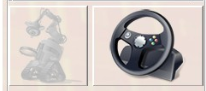
\includegraphics[width =0.8\linewidth]{robot_mode_change}}
\caption{Buttons for mode change}
\label{sec:NXJCC}
\label{fig:NXJCC}
\end{figure}

\paragraph{Acceptance criteria:}
When the users press the button of mode change, there is a window jumping out and write like "Do you want to change to the manual mode?" If the users press "yes", the robot will execute as manual mode. The same situation is also suitable for manual mode to automatic mode.
\paragraph{Source:}
 Minutes of the first client meeting 
\paragraph{Priority:}
High 


\subsection{R0012: User mode change}
\paragraph{Description:}
There are two modes can be switched: Client mode and Maintenance mode. In Client mode, this system allow client to control the robot by GUI, the client can use the robot to search the archaeological site and to find the hidden walls, blocks and the no-go zones. The client is not permitted to edit the setting of the robot, for example, the client is not allowed to change the speed setting and the Blue-tooth setting. In Maintenance mode, users can change the speed and the some other system settings.
\paragraph{Rationale:}
The Client mode is used by client, they do not need to understand the internal setting of the whole system. The robot is just a tool to finish its task. They are not permitted to change the internal setting, because sometimes clients do not understand the principle of this system, they may break the system due to some wrong operations for internal setting. Users with higher level skills and more experiences are allowed to change and improve the system, because this is our responsibility to make the system better.
\paragraph{Acceptance criteria:}
The default mode of the GUI is Client mode. If the client want to change to Maintenance mode, there will be a switch in the menu bar of the user interface. Then the users can change the internal settings like travel speed of the robot here.
\paragraph{Source:}
 Minutes of the first client meeting 
\paragraph{Priority:}
Low



\subsection{R0013: Save XML map file}
\paragraph{Description:}
The map need to be saved to the database. The GUI has a button to implement the save operation. 
\paragraph{Rationale:}
The robot is required to walk on any kind of maps, so the host system should be able to save more maps into the database. So we need to add a button in main GUI to control the save operation.
\paragraph{Acceptance criteria:}
When the robot finish the survey of the site, if users want to save the map, they can press the saving button to achieve it.  Then this finished map will be saved in the database. If the map is too big to survey in one session, users can save the map temporarily and continue mapping from where it left off next time.
\paragraph{Source}
 Project Description 2.1
\paragraph{Priority:}
High




\subsection{R0014: Load XML map file}
\paragraph{Description:}
The map need to be loaded from the database. The main GUI has a button to implement the load operation. 
\paragraph{Rationale:}
The robot is required to walk on any kind of maps, so the host system should be able to load more maps from database by clients. With the load operation users can continue mapping from where it left off.  So we need to add a button in main GUI to control the load operation.
\paragraph{Acceptance criteria:}
Wen users press the loading button, there is a window jumping out and you can choose the map from the database. They can check the mapping result of every map by using load operation.
\paragraph{Source}
 Project Description 2.1
\paragraph{Priority:}
High


\subsection{R0015:Show System information}
\paragraph{Description:}
The GUI will show the details of the whole system which include the speed of the robot, the battery status, the mode is selected and the Blue-tooth connection status.
\paragraph{Rationale:}
It is clearer to check the system when everything of it is put on the GUI. The user can control the system via GUI.
\paragraph{Acceptance criteria:}
The GUI will show the details of the system. All information must be real time.
\paragraph{Source:}
Minutes of the first client meeting.
\paragraph{Priority:}
Medium


\subsection{R0016: Boundaries of map}
\paragraph{Description:}
The survey map is not infinite extension, so we should set the boundaries correctly. The boundaries is the farthest way the robot can go to.
\paragraph{Rationale:}
According to the requirement of the description, the map should have boundaries so that the robot will not go outside of the survey map. The robot will only survey inside the boundary.
\paragraph{Acceptance criteria:}
when the robot reaches the boundaries, it will ignore receiving the forward command. That means if the robot is facing to a boundary, it will stop moving no matter how many time the user press "move forward". The user can only turn right, left and move backward.
\paragraph{Source:}
 Introduction of Project Description.
\paragraph{Priority:}
Low


\subsection{R0017: Mini map}
\paragraph{Description:}
This system shall have a mini map to show all the details of the map robot surveyed. All map details are demonstrated on the mini map. 
\paragraph{Rationale:}
Mini map is an efficient tool to demonstrate the general searching map. The map is allowed to be "zoom in" and "zoom out", it is necessary to demonstrate all map informations and robot's position on the mini map, which is convenient for the client to detect the detail information of the whole searching process.    
\paragraph{Acceptance criteria:}
The mini map displays all information of the map. The mini map is also able to be used to detect the position of the robot, the green grid in the mini map represents the robot. The complete mini map displays below:
\begin{figure}[ht]
\centering
\setlength\fboxsep{2pt}
\setlength\fboxrule{0.2pt}
\fbox{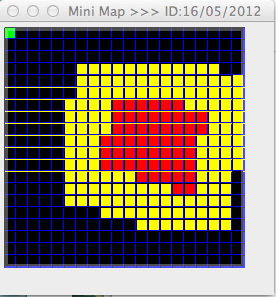
\includegraphics[width =0.4\linewidth]{minimap}}
\caption{The complete mini map}
\label{sec:NXJCC}
\label{fig:NXJCC}
\end{figure}

\paragraph{Source:}
Minutes of the 7th client meeting.
\paragraph{Priority:}
Low


\subsection{R0018: Keyboard short-cut}
\paragraph{Description:}
The user is allowed to operate the GUI by using the shortcut key from keyboard, which is more convenient for client's using.    
\paragraph{Rationale:}
We are willing to make the operation more easily. So we add the shortcut operation for our GUI.  
\paragraph{Acceptance criteria:}
Client is allowed to operate the GUI by keyboard. The specific shortcut keys display below:
\begin{figure}[ht]
\centering
\setlength\fboxsep{2pt}
\setlength\fboxrule{0.2pt}
\fbox{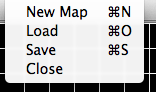
\includegraphics[width =0.4\linewidth]{shortcut1}}
\caption{The shortcut key1}
\label{sec:NXJCC}
\label{fig:NXJCC}
\end{figure}
\begin{figure}[ht]
\centering
\setlength\fboxsep{2pt}
\setlength\fboxrule{0.2pt}
\fbox{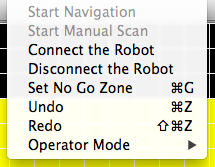
\includegraphics[width =0.4\linewidth]{shortcut2}}
\caption{The shortcut key2}
\label{sec:NXJCC}
\label{fig:NXJCC}
\end{figure}
\pagebreak
\paragraph{Source:}
Internal meeting discussion
\paragraph{Priority:}
Low


\section{Emergency handle}
\subsection{R0016: Handle entering the no-go zone by accident}
\paragraph{Description:}
For preventing some unanticipated situation, we set the Emergency Handle operation. When some accidents happen, users need to press Emergency Handle button.
\paragraph{Rationale:}
We must set some operation to deal with some unexpected situation, which is a necessary method to protect the whole robot system. 
\paragraph{Acceptance criteria:}
When the users press the Emergency Handle button, the robot will stop immediately and wait for the further command. For example, the robot has to stop at the boundary of the no-go zone. 
\paragraph{Source:}
 Minutes of the first client meeting 
\paragraph{Priority:}
High  


\subsection{R0017: Handle loss of communication}
\paragraph{Description:}
This system shall have the ability to handle a communication loss situation by stopping the robot immediately to ensure the safety of the robot. Also an error message will be shown on the main GUI in order to let users notice that the connection is lost. 
\paragraph{Rationale:}
A connection loss could cause operation fail or even broken the robot. In order to improve the entire operation's safety and efficiency, we add this requirement into our emergency handling procedures. 
\paragraph{Acceptance criteria:}
When a connection loss happen, the robot should stop operation immediately to avoid further damage, a error dialogue box shall appeared on the host machine waiting for further operation.
\paragraph{Source:}
Minutes of the first client meeting.
\paragraph{Priority:}
Medium


\subsection{R0018: Handle battery failure}
\paragraph{Description:}
This system shall be able to handle emergencies which include battery hardware failure, battery overheat and battery out of power.
\paragraph{Rationale:}
The robot should operate under sufficient energy at any time. However, There may be some cause to a battery failure such as faulty batteries and external damage to the battery. Such failure could cause connection loss and inaccurate information. 
\paragraph{Acceptance criteria:}
When the system detects the battery level is not enough for the robot to return to the start point, the robot should stop operation immediately and the host machine shall trying to reconnect the robot. if the reconnection failed, a error dialogue box shall appeared on the host machine waiting for further operation.
\paragraph{Source:}
Minutes of the first client meeting.
\paragraph{Priority:}
Medium

		
		   

% System Features %
\pagebreak
\chapter {System Features}
\section {Manual Control}
\subsection {Description and Priority}

The operator needs to hold the directional buttons on the Graphical User interface to control the movement of the robot and release it to stop. To change speed, the operator can select the appropriate speed on the slider bar. It is essential that the functions are implemented in the system to
move the robot to the starting point safely.\\ \\
Priority: High

\subsection {Stimulus/Response Sequences}

The operator has to select manual mode to enter manual control. The buttons in the
`Control' tab is then highlighted and is ready to use. The operator selects the appropriate speed by
moving the slider bar before holding on a directional button. The host software will send a PC packet
with the latest speed setting and the direction to the robot, moving the robot in the
indicated direction.

\subsection{Functional Requirements}


The manual control implements requirement R0001, R0002, R0003, R0010.\\ \\
The functional requirements of the manual control are as follows:
\begin{itemize}
	\item The GUI includes a "Control" panel that has directional buttons of moving
	forward, moving backwards, rotating left and rotating right.
	\item The "Control" panel also has a sliding bar that toggles the speed setting from 0 to 10. A speed setting of 0 halts the movement of the robot while the speed setting of 10 set the fastest possible speed for the robot. 
	\item If the robot enters a no-go zone , an emergency mechanism is triggered.
\end{itemize}

%The robot can enter external object even if under manual control%

\section {Automatic Control}
\subsection {Description and Priority}
The host software comes with an automatic navigation algorithm. The robot has a light sensor to detect a hidden wall and an ultrasonic sensor for detecting an obstacle object. Each time a wall is encountered by the robot, the robot sends a request to the host software controller to record the position and decide on the best possible path to take. The new generated path is then reflected on the GUI while the controller sends back the new path in a PC packet to the robot.\\ \\
The navigation system may start with either a new, partial or completed map. In any case, the map
will contain information for the starting position of the robot, obstacles and hidden walls\\ \\
Priority: High


\subsection {Stimulus/Response Sequences}

When the robot set on the starting position of the survey area , the operator has the option to switch to Auto Mode. This function disables Manual Controls while enabling the usage of the start and stop buttons. At this point, the operator can press the start button which causes the host software to initialise the robot with the starting position coordinates and an initial generated path. The robot then follows this path till it encounters an obstacle, then making change to map and requesting a new path.

\subsection {Functional Requirements}
The automatic path Finding navigation implements requirements  R0003, R0004, R0005, R0006,
R0007, R0009, R0011.\\ \\
The GUI contains a start and a stop button for Auto Mode. If the user push a start button, a map is to be generated and be displayed on screen.


\section{Graphical User Interface}
\subsection {Description and Priority}
The GUI serves as an interaction platform among the operator, the robot and the survey area.\\ \\
All controls are made available to the operator through the GUI. The GUI also includes executing
either automatic or manual robot control. In addition, the GUI provides a visual interpretation of the area to the operator in the form of a writeable XML map. As the robot makes its exploration, any objects encountered by the robot is displayed on the GUI. Lastly, the robot's status such as coordinates, speed is shown at the bottom of the GUI.\\ \\
Priority: High


\subsection{Stimulus/Response Sequences}

There are various components of the GUI that the operator can access:

\begin{itemize}
	\item The tool bar on top of the GUI - The operator has the ability to load map, save map and save as map through the "File" header. If the "Robot" header is accessed, the operator could connect and disconnect the robot. Under the "View" header, the grid and path taken by the robot can be toggled on and off. As for the last header named "System", the operator has the option to exit the system.
	\item The map interface and map editor - The map interface displays a loaded XML map which illustrates the survey area. A map editor is provided for the operator to add and remove no-go zones. 
	\item Manual mode - When the operator selects manual mode, he has access to the manual controls of the robot under the "Control" tab. Manual controls include moving the robot and altering the speed settings. 
	\item  Auto mode - Auto mode is used when the robot is placed at a designated start position in the survey area. When the operator selects auto mode, the manual functions are disabled immediately. If the start button is pressed, the robot will commence autonomous mapping. At any time the operator can click on the stop button to halt the operation. 
	\item Robot status -The status displays the robot's coordinates, the current mode, the speed of movement, connection and battery strength.
	\item Mini map - The mini map is used to display the general information of the map and the current position of the robot.
\end{itemize}

\subsection{Functional Requirements}

The graphical user interface implements requirements R0007, R0008, R0009, R0010, R0011

\begin{itemize}
	\item Directional buttons and speed toggle are needed for the manual mode.
	\item A start and a stop button are required for the auto mode.
	\item A mode switch is required.
	\item The GUI must support the functions of loading and saving a map.
	\item No-Go zones can be edited.
	\item The map must display the wall if the robot discovers one.
	\item The robot status must be displayed.
\end{itemize}

\section{Load XML File}
\subsection{Description and Priority}
The system is required to accept/load Extensible Mark-up Language. Since the map is saved in XML files, it is significant to load the map from XML file. The XML files includes all map information(the coordinate, hidden walls, obstacles and no go zones ) which need to display on GUI.\\ \\
Priority: High
\subsection{Stimulus/Response Sequences}
As the requirement from client, the map should be built in the XML format therefore the system needs to be able to interpret these XML map files and display the map and its features to the client. 

\subsection{Functional Requirements}
the Load XML File implements requirements R0011
\begin{enumerate}
\item Extract all informations from each XML file, get the locations of the hidden walls, obstacles and no go zones.
\item Get the start position of the robot on the map  
\end{enumerate}
\section{Save XML File}
\subsection{Description and Priority}
The system is required to save the current map with all informations(hidden walls, obstacles and no go zones) in one XML file.\\ \\
Priority: High
\subsection{Stimulus/Response Sequences}
As the requirement from client, the map should be built in the XML format and save all informations in XML file, which is convenient for operator to stop operation and restart operation at any time.
\subsection{Functional Requirements}
the Save XML File implements requirements R0011
\begin{enumerate}
\item Save all informations to a XML file, include all the locations of the hidden walls, obstacles and no go zones informations.
\item Store the start position of the robot on the map  

\end{enumerate}


\section{Use Cases}
\subsection{General Use Case}
\paragraph{UC001: Operating the robot in manual mode}
UC001 is associated with section 4.1 - Manual control as well as R0001.
	\begin{itemize}	
		\item \textbf{Description:} The use case demonstrates the operation of the robot under complete manipulation of the operator.
		\item \textbf{Goal:} The objective of this use case is to ensure that the robot under the control of the operator
	\end{itemize}
	\textbf{Flow of Events:} The robot is placed in an arbitrary position of the map while
	the operator is controlling the robot through Blue-tooth.
	\begin{itemize}
		\item The operator opens a new map which is set as unexplored map.  
		\item The operator switches the robot on and runs the program. He then executes the GUI to connect with the robot. Next, he selects the manual mode.
		\item The control buttons are highlighted to imply that it is ready for use. The operator selects the appropriate speed by using the slider bar.
		\item The operator then holds down the directional key to move the robot till it reaches the destination.	
		\item The map will be drawn synchronously on the GUI as the movement of the robot.   	
	\end{itemize}
	\textbf{Preconditions:}
	\begin{itemize}
		\item	The robot batteries are charged and the robot is working properly.
		\item	The GUI must be working correctly.
		\item	The Blue-tooth connection operates normally.
		\item	An appropriate XML formatted map must be loaded. This map may be a new, partial or completed map.
		\item The operator must have already chosen the Manual Control mode. 
	\end{itemize}
	\textbf{Postconditions:}
	\begin{itemize}
		\item The robot reaches the destination safely.
		\item The robot is able to avoid all external objects and no go zones.
	\end{itemize}


\paragraph {UC002: Operating the robot in auto scan mode}
	\begin{itemize}
		\item \textbf{Description:} Under the supervision of the operator, the robot commences autonomous mapping from a given starting point of the survey area.
		\item \textbf{Goal:} The end result of this use case is achieved when the robot has successfully mapped all the points in the area.
	\end{itemize}
	\textbf{Flow of Events:} Using auto controls, the robot is moved onto the starting position of the
survey area. Like UC001, the operator supervises the robot through the host machine.
	\begin{itemize}
		\item The operator opens a new map which is set as unexplored map.  
		\item The operator ensures switched on the robot, executing the program. He then
opens the host machine to run the GUI. The operator connects the robot through Blue-tooth, after the robot is connected, selecting the automatic mode.
		\item The operator select the ``Option'' in the menu bar, then click ``Start Navigation'' to start auto navigation and scan.
		\item Without being interrupted, the robot moves on its own till it finishes mapping. The actions are now determined by the controller in the host machine.
		\item The map will be drawn synchronously on the GUI as the movement of the robot.  
		\item If the operator wishes to halt the progress of the autonomous search, he can stop the operation via ``Stop Operation'' in the ``Option''. 
    \item If operator save the map to XML file by choosing: ``File'', then choose ``Save'' or save the map through keyboard short cut ``Control+S''.
	\end{itemize}
	\textbf{Preconditions:}
	\begin{itemize}
		\item The robot batteries are charged and the robot is working properly.
		\item The GUI on the host machine must be running correctly.
		\item The connection between robot and host machine is stable.
		\item An appropriate XML formatted map can be loaded. This map may be a new, partial or
completed map.
		\item The robot is under the auto scan mode.
	\end{itemize}
	\textbf{Postconditions:}
	\begin{itemize}
		\item The robot finished mapping completely and safely.
	\end{itemize}


\paragraph{UC003: Operating the robot in manual scan mode} % (fold)
\label{par:uc003_operating_the_robot_in_manual_scan_mode}
\begin{enumerate}
    \item \textbf{Description:} Under the command of the operator, the robot can scan the map by operator's command.
    \item \textbf{Goal:} When robot is done with the auto scan, if operator wish to scan the part which robot missed on the map, manual scan mode can be activated and robot will follow operator's command finishing the scan of the map.
  \end{enumerate}
  \textbf{Flow of Events:} 
  \begin{itemize}
  	\item Operator makes sure the GUI is connected to the robot.
  	\item Operator makes sure the robot is not in auto scan mode and waiting for command.
  	\item Operator makes sure robot is on the map which GUI's map panel is currently showing, and robot is in the right position which is the ``current pixel'' on the map panel. If not, operator can move the robot to that position via manual control.
  	\item Operator choose ``Start Manual Scan'' in ``Option'' to start manual scan.
  	\item Operator shall be allowed to control the robot scan the map using ``Up'', ``Down'', ``Left'', and ``Right''.
  	\item When Operator is down with the manual scan, operator can using manual control to control the robot back to the start point.
  	\item Operator can save the map into a XMl file in any stage above.
  \end{itemize}
	\textbf{Preconditions:}
  \begin{itemize}
    \item The robot batteries are charged and the robot is working properly.
    \item The GUI on the host machine must be running correctly.
    \item The connection between robot and host machine is stable.
    \item An appropriate XML formatted map can be loaded. This map may be a new, partial or
completed map.
    \item The robot is under the manual scan mode.
  \end{itemize}
  \textbf{Postconditions:}
  \begin{itemize}
    \item The robot back to the starting point by operator's command.
  \end{itemize}
  % paragraph uc003_operating_the_robot_in_manual_scan_mode (end)
\pagebreak

\subsection{Exceptional Use Cases}
\paragraph {UC004: Loss of communication signal}
	\begin{itemize}
		\item \textbf{Description:} The process details on the steps taken by the robot in the event if the Blue-tooth communication link is broken between the host software and the robot.
		\item \textbf{Goal:} The robot stops operation and operator informed by the host.
	\end{itemize}
		\textbf{Flow of Events:}
	\begin{itemize}
		\item During manual or autonomous mode, communication between host software and
robot is lost.
		\item The robot stops at its current position.
		\item The robot will remain at its current position and wait for the rescue. At the same time, error message should appear to host machine to notify the operator.
	\end{itemize}
	\textbf{Preconditions:}
	\begin{itemize}
		\item The robot is having a connection with the host software.
	\end{itemize}
	\textbf{Postconditions:}
	\begin{itemize}
		\item The robot should stop immediately
		\item The error message should appear to the GUI to inform the operator to rescue the robot.
	\end{itemize}
\pagebreak

\paragraph {UC005: Low battery level handle}
	\begin{itemize}
		\item \textbf{Description:} The processes details taken when robot's battery level is running low(less then 20 percent).
		\item \textbf{Goal:} Robot back to the start point and map was successfully saved.
	\end{itemize}
		\textbf{Flow of Events:}
	\begin{itemize}
		\item Toe robot's battery level is lower then 20 percent.
		\item A message dialogue pop on the host machine's screen and inform operator that robot's battery level is under 20 percent, also recommend user to save the map and stop the operation.
		\item Operator stops the robot's operation, save the map into XML file, and control the robot via manual control back to the starting point.
	\end{itemize}
	\textbf{Preconditions:}
	\begin{itemize}
		\item The robot's battery level is lower then 20 percent.
	\end{itemize}
	\textbf{Postconditions:}
	\begin{itemize}
		\item Message dialogue is shown to operator.
		\item Robot back to the starting point by operators command, map was successfully saved.
	\end{itemize}
\pagebreak
 

% External Interface Requirements %

\chapter{External Interface Requirements}

\section{User Interface}

\begin{figure}[ht]
\centering
\setlength\fboxsep{2pt}
\setlength\fboxrule{0.2pt}
\fbox{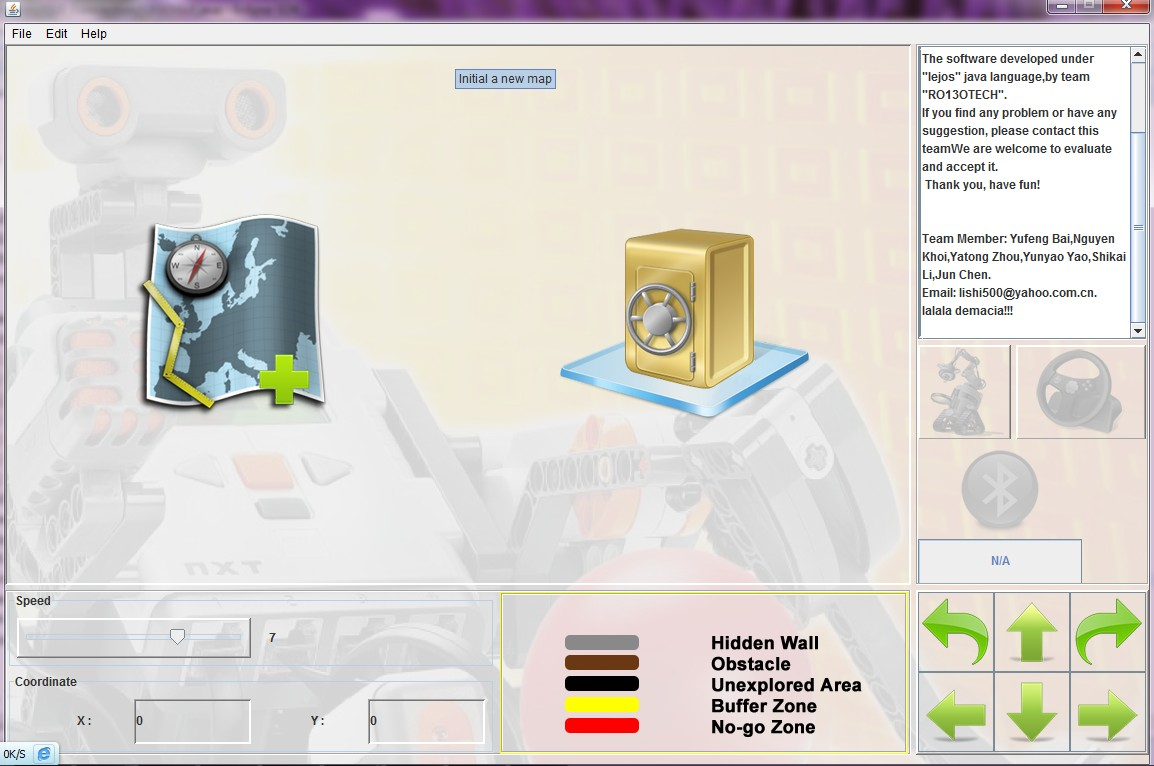
\includegraphics[width =0.6\linewidth]{newGUI}}
\caption{Overview of the graphic user interface}
\label{sec:GUI}
\label{fig:GUI}
\end{figure}

\begin{figure}[ht]
\centering
\setlength\fboxsep{2pt}
\setlength\fboxrule{0.2pt}
\fbox{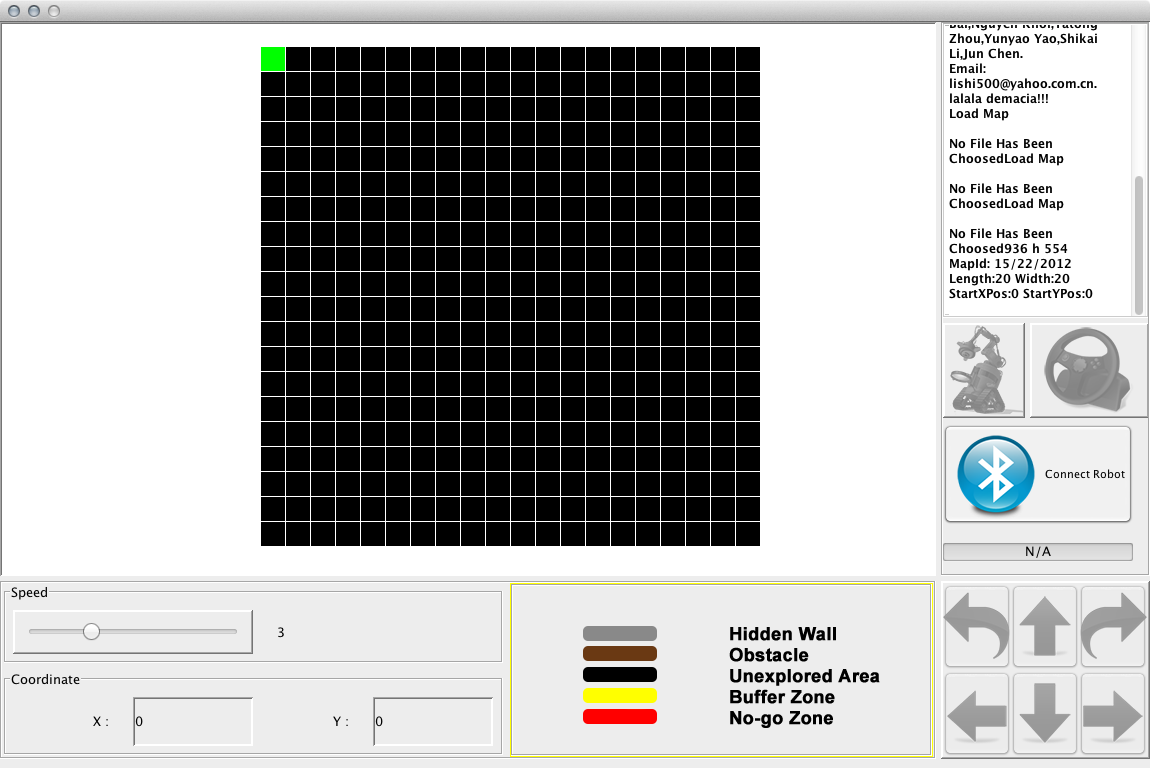
\includegraphics[width =0.6\linewidth]{newGUI_map}}
\caption{Overview of the graphic user interface with map}
\label{sec:GUI}
\label{fig:GUI}
\end{figure}
\pagebreak
\begin{figure}[ht]
\centering
\setlength\fboxsep{2pt}
\setlength\fboxrule{0.2pt}
\fbox{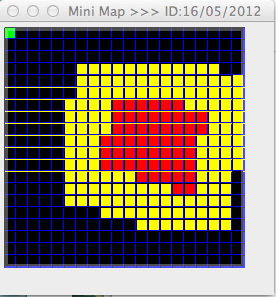
\includegraphics[width =0.6\linewidth]{minimap}}
\caption{Overview of the graphic user interface with mini map}
\label{sec:GUI}
\label{fig:GUI}
\end{figure}
The GUI is a Java-Based Program, which is used to control robot from the host computer. 
\begin{enumerate}
\item The UI Window has a menu bar on the top. The menu bar contains three menus: "File", "Option" and "Help". The "File" menu contains options to create, load and save map. The "File" menu also allow the operator to close the GUI. The "Option" menu has some functions to connect and disconnect the robot, change the operation mode and set no go zones. The "Option" also allows the operator to implement the "redo" and "undo" operation. "Help" menu contains an "about" item which shows the information of the software and the developing team. The "Help" menu also allow operator to set the battery level. 
\item The main desk panel contains the map display area with one icon which is represented as the robot. When the robot detects on the map, the icon will move on the map of GUI and demonstrate the items(include hidden walls, obstacles and no go zones) on the map of GUI using the grids of different colour.
\item Right side panel contains log information, auto/ manual mode switch buttons, battery and Blue-tooth connection state, and direction control buttons. 
\item Bottom panel contains current coordinate of robot in map, the speed slider bar and some related icons for items on the map. 
\item There is also a mini map window generating beside the main GUI, which is used to demonstrate the general information of the map and the robot position. 
\end{enumerate}

\pagebreak

\section{Hardware Interfaces}


\begin{figure}[ht]
\centering
\setlength\fboxsep{2pt}
\setlength\fboxrule{0.2pt}
\fbox{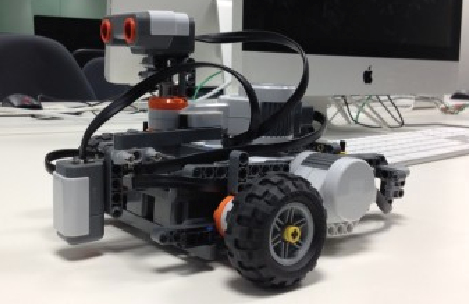
\includegraphics[width =0.8\linewidth]{robot_interface}}
\caption{Hardware interfaces contains robot body (robot interface)}
\label{sec:GUI}
\label{fig:GUI}
\end{figure}

The robot has these four main interfaces:
\begin{itemize}
	\item{Blue-tooth connection:}\\
	This part is the wireless communication device and data transfer device between user and robot. 
	\item{Light sensor:}\\
	Light sensor can detect the hidden wall on the map according to the different colours of the grids.
	\item{Ultrasonic sensor:}\\
	Ultrasonic sensor is the device on the robot which looks like two "eyes", it has the function like eyes as well. This device can sense the obstacle in front of the robot, and it will warn the user if the robot is closing to the barrier. It can also let the robot stop through software when danger located in front of the robot.
	\item{USB interface:}\\
	USB interface has the same function as the Blue-tooth. The difference is the data transfer and communications are both via a USB cable.
\end{itemize}
\pagebreak
\section{Software Interfaces}
Any machine (Mac/Windows/Linux) installed Java SE6 can run the software. GUI supports the leJOS NXJ PC API and leJOS NXJ API documentation can be operated by the user, to implement this, the machine are required capable at either Blue-tooth or USB connection. Real maps can be created, load and save map file through the GUI.


\section{Communications Interfaces}
Blue-tooth (wireless) or USB (cable) connection can be used to connect the host machine with the robot.  Files manipulation and other communication can be made through LeJOS NXJ Control Centre like this(optional): 

\begin{figure}[ht]
\centering
\setlength\fboxsep{2pt}
\setlength\fboxrule{0.2pt}
\fbox{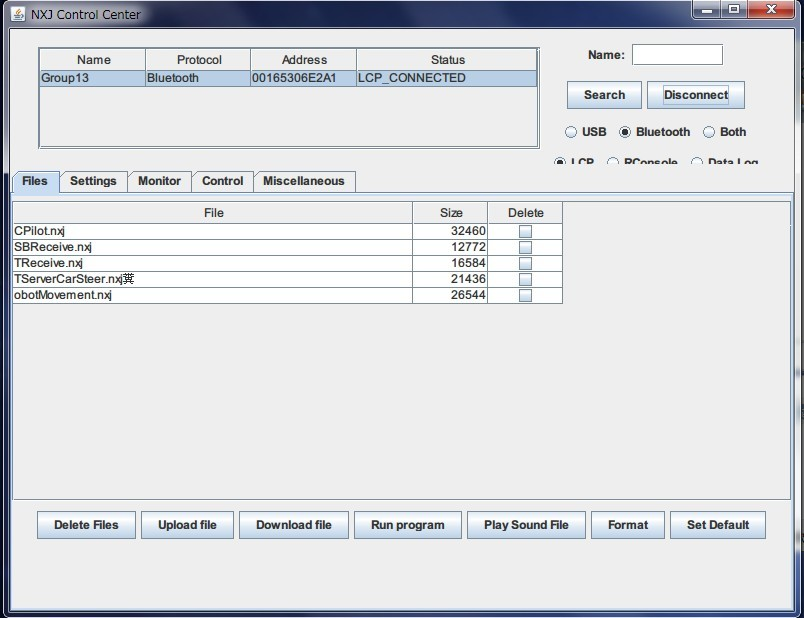
\includegraphics[width =0.8\linewidth]{NXJ_Control_Center}}
\caption{NXJ Control Center}
\label{sec:NXJCC}
\label{fig:NXJCC}
\end{figure}
With this program, basic connection can be made easily between host computer and robot. 
We can delete and upload testing source codes via either Blue-tooth or USB cable.
\pagebreak


% Other Nonfunctional Requirements %

\chapter{Other Non-functional Requirements}


\section{Performance Requirements}

\subsection{N0001: Time Performance}
\paragraph{Description:}
The robot must be able to scan the whole map and detect all the elements on that map within a adequate amount of time according to the size of the map. The time is 20 minutes approximately. 
\paragraph{Rationale:}
The robot need to finish all tasks in limited time which is used to make sure the power of battery is enough to support the whole process. For getting the maxim battery power, we charge the battery to get the maxim value and then test how long it is able to be used. When we get the accurate time value, we have to make sure the robot finishes all tasks in this certain time.   

\paragraph{Priority:}
Low

\subsection{N0002: Accuracy Performance}
\paragraph{Description:}
\begin{enumerate}
\item The movement of the robot is required to be implemented correctly and accurately. When we check the movement of the robot, we are required to make sure the robot is able to rotate and move in right angle and distance.
\item The position of the robot is required to demonstrate on the GUI accurately.
\item The robot is required to distinguish the hidden walls, obstacles and no go zones.
  \end{enumerate}
\paragraph{Rationale:}
\begin{enumerate}
\item For getting the accurate angle and distance, we build the 90 degrees, 180 degrees and 360 degrees angle in internal meeting, then keep testing which value is able to get all these degrees in algorithm.
\item For getting the position of robot in GUI, we decide to use the icon of the robot to move on the map in grid as the unit and make sure the icon of robot is on the boundary line of the grid all the time.
\item For distinguishing the hidden walls, obstacles and no go zones, we will use different colour to represent the different items of map. 
\end{enumerate}
\paragraph{Priority:}
Medium

\section{Safety Requirements}

\subsection{N0003: latency}
\paragraph{Description:}
Robot is able to give a response to the command in a response time. Normally, this time is 0.1 second.
\paragraph{Rationale:}
Response time could be extremely important when the robot is in a dangerous situation and emergency stop needs to be carried out.
\paragraph{Priority:}
High

\subsection{N0004: Component Safety}
\paragraph{Description:}
The component of the robot is required to keep safely to make sure that no parts become lose and fall off during the whole mission. 
\paragraph{Rationale}    
A missing component of the robot will affect the function of the robot and may cause the damage of the robot. As the result, it is necessary to protect the completion of the robot.
\paragraph{Priority:}
High
\subsection{N0005: Robot Design}
\paragraph{Description:}
The user will use the robot in some unexpected environment, so we need to design the robot to work properly in any environment. 
\paragraph{Rationale:}
It is new essential to build one firm robot. The robot should be designed sensibly and stably so that it will not be effected by the change of environment. 
\paragraph{Priority:}
High

\section{Security Requirements}
\subsection{N0006: Data Security}
\paragraph{Description:}
Data is required to store in the SVN repository, the specific data is forbidden to be exposed to others. To ensure this, the team member is not allowed to reveal their SVN password. The project manager will check the SVN frequently to make sure the data is not damaged by others.
\paragraph{Rationale:}
This strategy is used to make sure nobody steals or copy our data.
\paragraph{Priority:}
High
\subsection{N0007: Robot Security}
\paragraph{Description:}
Robot is required to store in the locker, the robot is forbidden to be borrowed by others. To ensure this, the team will choose one member to keep the key. If one team member want to bring the robot home, he have to get agreement from project manager, the key keeper does not have right to lend the key to others without permission, even the team member. 
\paragraph{Rationale:}
This strategy is used to make sure nobody steals or damage the robot.
\paragraph{Priority:}
High

\section{Software Quality Attributes}
\subsection{N0008: Quality of code}
\paragraph{Description:}
It is essential to write the code clearly. The format and the layout of the codes need to be written in same standard. The standard is made after negotiating in internal meeting.
\paragraph{Rationale:}
This is used to make the codes much easier to read by client and other developers.
\paragraph{Priority:}
Medium

\subsection{N0009: Program Testability}
\paragraph{Description:}
The program is required to be tested by all developers in any time when needed. 
\paragraph{Rationale:}
Every developers is required to test the program to make sure we can fix more bugs before demonstrating to client. This is an efficient way to make the project better.
\paragraph{Priority:}
High

\chapter{Other Requirements}
\section{Poster}
Developers are required to design and build one poster with brief personal information and skills on every team members. The poster is used to introduce the team members to client.

\section{SPMP}
Developers are required to write a Software Project Management Plan document. This document include a description of the risk management and work plan. The project plan should also provide estimated completion times and required resources for each tasks.

\section{SDD}
The purpose of Software Design Document is to provide the overall architectural model of the system and the component details. The diagrams also need to be included in this project.


\section{UM}
User Manual is used to show how to operate the system by the client. This document also demonstrates some important notices which are used to remind client how to avoid some risk operation. 
\section{TR}
Test report is used to show some test case to client, which is also used to show the quality of the product. 


\pagebreak

% Appendicies %
\newpage
\appendix

\pagebreak

\chapter{Glossary}

\textbf{Automatic Mode}:  Mode of operation, completely controlled by robot and host machine, without human input of movements. \\
\\ \textbf{Blue-tooth}: Wireless connection used to communicate between robot and host machine.\\
\\ \textbf{Explored Area}: The area that robot have inspected, which allows robot to travel safely.  \\
\\ \textbf{Gird}: A size of 50mm*50mm area in map, which contains 4 pixels. Each gird can be labelled as explored, unexplored, or no-go.\\
\\ \textbf{GUI}: Graphical User Interface. Displays the map panel, control panel and status panel.\\
\\ \textbf{Light Sensor}: Sensor used to detect hidden walls within the site, located at the front of the robot. The sensor returns the distance of the object.\\
\\ \textbf{Manual Mode}: Mode of operation. Movements controlled directly through operator.\\
\\ \textbf{no-go zone}: A zone predefined is forbidden for the robot to enter. \\
\\ \textbf{Pixel}: A size of 25mm*25mm area in map, defined as the smallest resolution, which is also the smallest area of hidden walls that robot can detect.  \\
\\ \textbf{SDD}: Software Design Document.\\
\\ \textbf{SEP}: Software Engineering and Project.\\
\\ \textbf{SPMP}: Software Project Management Plan.\\
\\ \textbf{Ultrasonic Sensor}: Sensor used to detect walls and obstacles within the site, located at the front of the robot. The sensor returns the distance of the object.\\
\\ \textbf{Unexplored Area}: The area that robot have not inspected, which can be considered dangerous.  \\
\\ \textbf{XML}: Extensible Mark-up Language. The map is saved as an XML file.\\





\end{document}

